%% abtex2-modelo-trabalho-academico.tex, v-1.8 laurocesar
%% Copyright 2012-2013 by abnTeX2 group at http://abntex2.googlecode.com/ 
%%
%% This work may be distributed and/or modified under the
%% conditions of the LaTeX Project Public License, either version 1.3
%% of this license or (at your option) any later version.
%% The latest version of this license is in
%%   http://www.latex-project.org/lppl.txt
%% and version 1.3 or later is part of all distributions of LaTeX
%% version 2005/12/01 or later.
%%
%% This work has the LPPL maintenance status `maintained'.
%% 
%% The Current Maintainer of this work is the abnTeX2 team, led
%% by Lauro César Araujo. Further information are available on 
%% http://abntex2.googlecode.com/
%%
%% This work consists of the files abntex2-modelo-trabalho-academico.tex,
%% abntex2-modelo-include-comandos and abntex2-modelo-references.bib
%%

% ------------------------------------------------------------------------
% ------------------------------------------------------------------------
% abnTeX2: Modelo de Trabalho Academico (tese de doutorado, dissertacao de
% mestrado e trabalhos monograficos em geral) em conformidade com 
% ABNT NBR 14724:2011: Informacao e documentacao - Trabalhos academicos -
% Apresentacao
% ------------------------------------------------------------------------
% ------------------------------------------------------------------------

\documentclass[
	% -- opções da classe memoir --
	11pt,				% tamanho da fonte
	openright,			% capítulos começam em pág ímpar (insere página vazia caso preciso)
	oneside,			% twoside para impressão em verso e anverso. Oposto a oneside
	a4paper,			% tamanho do papel. 
	% -- opções da classe abntex2 --
	%chapter=TITLE,		% títulos de capítulos convertidos em letras maiúsculas
	%section=TITLE,		% títulos de seções convertidos em letras maiúsculas
	%subsection=TITLE,	% títulos de subseções convertidos em letras maiúsculas
	%subsubsection=TITLE,% títulos de subsubseções convertidos em letras maiúsculas
	% -- opções do pacote babel --
	english,			% idioma adicional para hifenização
	french,				% idioma adicional para hifenização
	spanish,			% idioma adicional para hifenização
	brazil,				% o último idioma é o principal do documento
	]{abntex2}

\usepackage{abntex2-cefetmg-timoteo}

% ---
% PACOTES
% ---

% ---
% Pacotes fundamentais 
% ---
\usepackage{cmap}				% Mapear caracteres especiais no PDF
\usepackage{lmodern}			% Usa a fonte Latin Modern			
\usepackage[T1]{fontenc}		% Selecao de codigos de fonte.
\usepackage[utf8]{inputenc}		% Codificacao do documento (conversão automática dos acentos)
\usepackage{lastpage}			% Usado pela Ficha catalográfica
\usepackage{indentfirst}		% Indenta o primeiro parágrafo de cada seção.
\usepackage{color}				% Controle das cores
\usepackage{graphicx}			% Inclusão de gráficos
\PassOptionsToPackage{normalem}{ulem} % Para não usar sublinhado em referências bibliográficas
\usepackage{ulem}
\usepackage{multicol}
\usepackage{url}
% ---

%Trocar fonte para Arial ou Helvetica
%\usepackage{uarial}
\usepackage{helvet}
\renewcommand{\familydefault}{\sfdefault}

		
% ---
% Pacotes adicionais, usados apenas no âmbito do Modelo Canônico do abnteX2
% ---
%\usepackage{lipsum}				% para geração de dummy text
% ---

% ---
% Pacotes de citações
% ---
\usepackage[brazilian,hyperpageref]{backref}	 % Paginas com as citações na bibl
\usepackage[alf,abnt-thesis-year=both,]{abntex2cite}	% Citações padrão ABNT


%Outros pacotes

\usepackage{longtable}


%\setlrmarginsandblock{3cm}{2cm}{*}
%\setulmarginsandblock{3cm}{2cm}{*}
%\checkandfixthelayout


% --- 
% CONFIGURAÇÕES DE PACOTES
% --- 

% ---
% Configurações do pacote backref
% Usado sem a opção hyperpageref de backref
\renewcommand{\backrefpagesname}{Citado na(s) página(s):~}
% Texto padrão antes do número das páginas
\renewcommand{\backref}{}
% Define os textos da citação
\renewcommand*{\backrefalt}[4]{
	\ifcase #1 %
		Nenhuma citação no texto.%
	\or
		Citado na página #2.%
	\else
		%Citado #1 vezes nas páginas #2.%
		Citado nas páginas #2.%
	\fi}%
% ---


% ---
% Informações de dados para CAPA e FOLHA DE ROSTO
% ---
\titulo{lista 2 - aed ii\\  pseudo Geradores de Números Aleatórios }
\autor{José Geraldo Duarte Junior}
\local{Timóteo}
\data{2022}
\orientador{Gustavo Martins}
\coorientador{}
\instituicao{%
  Centro Federal de Educação Tecnológica de Minas Gerais
  \par
  Campus Timóteo
  \par
  Graduação em Engenharia de Computação
}
\tipotrabalho{Lista 1 - aed ii}
% O preambulo deve conter o tipo do trabalho, o objetivo, 
% o nome da instituição e a área de concentração 

%\preambulo{Proposta de pesquisa apresentada à Coordenação de Engenharia de Computação do Campus Timóteo do Centro Federal de Educação Tecnológica de Minas Gerais para obtenção do grau de Bacharel em Engenharia de Computação.}

\preambulo{Atividade apresentado ao professor Gustavo Martins, da disciplina de Algoritmo e Estrutura de Dados 2 do curso de Engenharia de Computação do Campus Timóteo do Centro Federal de Educação Tecnológica de Minas Gerais para aprovação na disciplina ofertada pelo mesmo.}

% ---

% ---
% Configurações de aparência do PDF final

% informações do PDF
\makeatletter
\hypersetup{
     	%pagebackref=true,
		pdftitle={\@title}, 
		pdfauthor={\@author},
    	pdfsubject={\imprimirpreambulo},
	    pdfcreator={LaTeX with abnTeX2},
		pdfkeywords={abnt}{latex}{abntex}{abntex2}{trabalho acadêmico}, 
		colorlinks=true,       		% false: boxed links; true: colored links
    	linkcolor=black,          	% color of internal links
    	citecolor=black,        		% color of links to bibliography
    	filecolor=black,      		% color of file links
		urlcolor=black,
		bookmarksdepth=4
}
\makeatother
% --- 

% --- 
% Espaçamentos entre linhas e parágrafos 
% --- 

% O tamanho do parágrafo é dado por:
\setlength{\parindent}{1.3cm}

% Controle do espaçamento entre um parágrafo e outro:
\setlength{\parskip}{0.2cm}  % tente também \onelineskip

% ---
% compila o indice
% ---
\makeindex
% ---

% ----
% Início do documento
% ----
\begin{document}

% Retira espaço extra obsoleto entre as frases.
\frenchspacing 

% ----------------------------------------------------------
% ELEMENTOS PRÉ-TEXTUAIS
% ----------------------------------------------------------
 \pretextual

% ---
% Capa
% ---
\imprimircapa
% ---

% ---
% Folha de rosto
% (o * indica que haverá a ficha bibliográfica)
% ---
\imprimirfolhaderosto*
% ---


% ---
% inserir lista de ilustrações
% ---

%%% no extra space before the entry, or in the LoF/LoT
% \setlength{\cftbeforechapterskip}{0pt plus 0pt} %afeta sumário, o que não desejo!
 \renewcommand*{\insertchapterspace}{} %afeta apenas lista de figuras e lista de tabelas, precisamente o que desejo!


\pdfbookmark[0]{\listfigurename}{lof}
\listoffigures*
\cleardoublepage
% ---

% ---
\pdfbookmark[0]{\listfigurename}{lof}
\tableofcontents*
\cleardoublepage
% ---



% ----------------------------------------------------------
% ELEMENTOS TEXTUAIS
% ----------------------------------------------------------
\textual

% ----------------------------------------------------------
% Introdução
% ----------------------------------------------------------
\chapter[Introdução]{Introdução}

%\chapter{Introdução}

	\begin{flushright}
		\textit{``Não existe resposta errada: \\ ela apenas não responde a essa pergunta''.\\
		Confia}
	\end{flushright}
	
	Quando empurramos ou puxamos um determinado objeto tentando movê-lo, percebemos que existe certa dificuldade para coloca-lo em movimento. Essa dificuldade deve-se à força de atrito, que é uma força que se opõe ao movimento de objetos que estão sob a ação de uma força. Ela age paralelamente à superfície de contato em sentido contrario a força aplicada sobre um corpo\cite{da2019estudo}.
	
	Neste documento também são trazidas informações sobre o desenvolvimento e uso de roldanas e polias. Analogamente, desde os séculos passados, com o avanço da tecnologia, houve a necessidade de que o esforço físico fosse empregado cada vez menos ou com menor grau de peso resultante para que se pudesse ter um rendimento maior nas ações de transportes e elevações de materiais ou de objetos pesados. Com isso, as roldanas, também chamadas de polias, são tipos de rodas utilizados em um sistema para direcionar a força feita sobre determinados objetos por meio de fios, cordas ou cabos, de modo que seja possível desviar a trajetória ou até mesmo levantá-los. As roldanas podem facilitar a realização de algumas tarefas, dependendo da maneira com que elas são interligadas. Dessa forma, existem dois tipos de polias: as polias fixas e as polias móveis\cite{site1}.

\chapter{Desenvolvimento}
\label{desenvolvimento}
%\chapter{Desenvolvimento}
\label{desenvolvimento}
\section{Remoção na SBB Sequencial}
    Iniciando o desenvolvimento da prática, as arvores foram criadas na IDE assim como os vetores de tamanhos diversos para armazenar os valores que serão inseridos na arvore. Porém, o Java não permite a criação de vetores em 10\textsuperscript{9} elementos, então todas as arvores criadas, foram geradas até 10\textsuperscript{7} elementos. A partir disso, foram utilizados métodos de inserção de dados da Pratica 3, desenvolvida anterior a esta, já que este trabalho trata-se de uma continuação direta com estudos sobre remoção.
    
    Aos dados selecionados para a remoção foram gerados utilizando a biblioteca interna do Java "Random", que permitiu gerar valores aleatórios entre 0 e n (n = quantidade de elementos), aumentando a taxa de sucesso para gerar valores validos para a remoção.
    Os dados apresentados a seguir inicialmente trazem os resultados do tempo de execução da da remoção de 5\% de elementos aleatórios de arvores de diferentes tamanhos que receberam seus valores de forma ordenada:
    
    \begin{center}
        \begin{tabular}{| l | r |}
            \hline
            Quantidade de elementos & Tempo em Nanossegundos\\
            \hline
            10\textsuperscript{3} & 820800\\
            10\textsuperscript{5} & 2165600\\
            10\textsuperscript{7} & 119273300\\
            \hline
        \end{tabular}
    \end{center}

        \begin{center}
            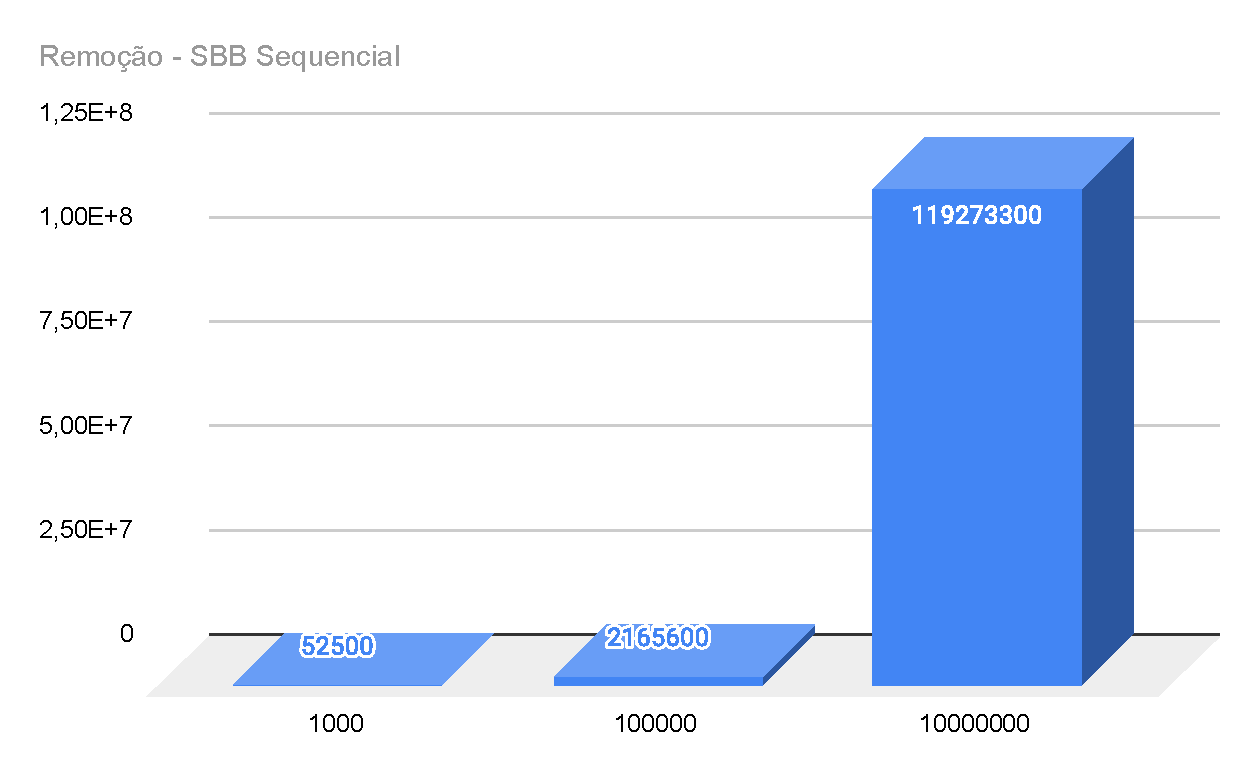
\includegraphics[scale=0.8]{Trabalho AED/fig/chart.pdf}
            \label{fig:Grafico 1}
        \end{center}

\section{Remoção na SBB Randômica}

Para a remoção de elementos aleatórios desta arvore foi gerado um vetor com valores aleatórios utilizando um gerador congruencial pseudo aleatório com os seguintes parâmetros:
        \begin{center}
        Semente = 0;
       
        Modulo = 1073741824;
       
        Multiplicador = 843314861;
       
        Incremento = 453816693;
        \end{center}

Estes parâmetros também foram utilizados na inserção, então é certo que os mesmos estarão na arvore, mas não foram removidos na mesma ordem que foram inseridos, e sim de forma aleatória também.

Logo os dados apresentados a seguir trazem os resultados do tempo de execução da da remoção de 5\% de elementos aleatórios de arvores de diferentes tamanhos que receberam seus valores de forma aleatória:

\begin{center}
        \begin{tabular}{| l | r |}
            \hline
            Quantidade de elementos & Tempo em Nanossegundos\\
            \hline
            10\textsuperscript{3} & 208600\\
            10\textsuperscript{5} & 3452300\\
            10\textsuperscript{7} & 822413400\\
            \hline
        \end{tabular}
    \end{center}
    
    \begin{center}
            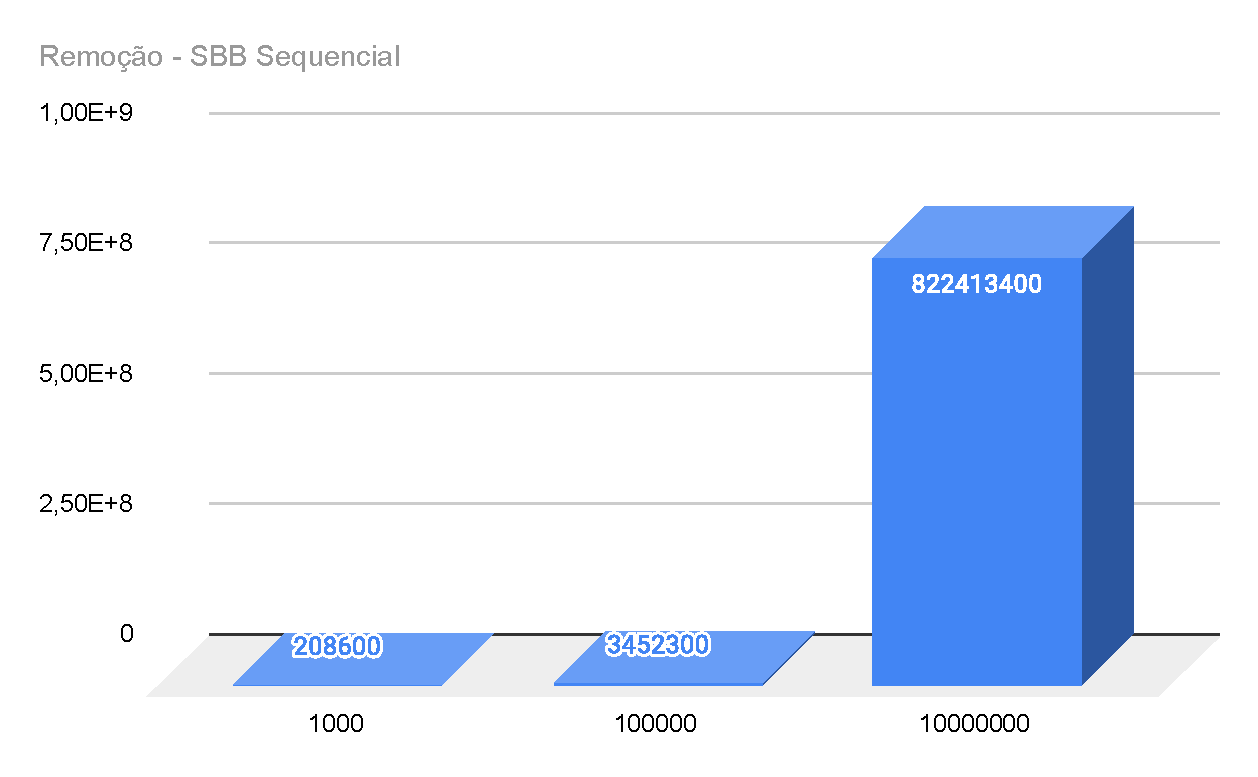
\includegraphics[scale=0.8]{Trabalho AED/fig/chart (1).pdf}
            \label{fig:Grafico 2}
    \end{center}
    
\section{Remoção na SBB Balanceada}
Para a remoção de elementos de dentro da arvore balanceada a logica utilizada segue a mesma da arvore sequencial, já que os valores inseridos na mesma estão entre 0 e n (n = quantidade de elementos), porem foram inseridos em uma condição especial que força a arvore a ser formada de já balanceada, como foi visto na atividade pratica 3.

Logo os dados apresentados a seguir trazem os resultados do tempo de execução da remoção de 5\% de elementos aleatórios de SBBs de diferentes tamanhos:

    \begin{center}
        \begin{tabular}{| l | r |}
            \hline
            Quantidade de elementos & Tempo em Nanossegundos\\
            \hline
            10\textsuperscript{3} & 11700\\
            10\textsuperscript{5} & 769600\\
            10\textsuperscript{7} & 149937300\\
            \hline
        \end{tabular}
    \end{center}
    
    \begin{center}
            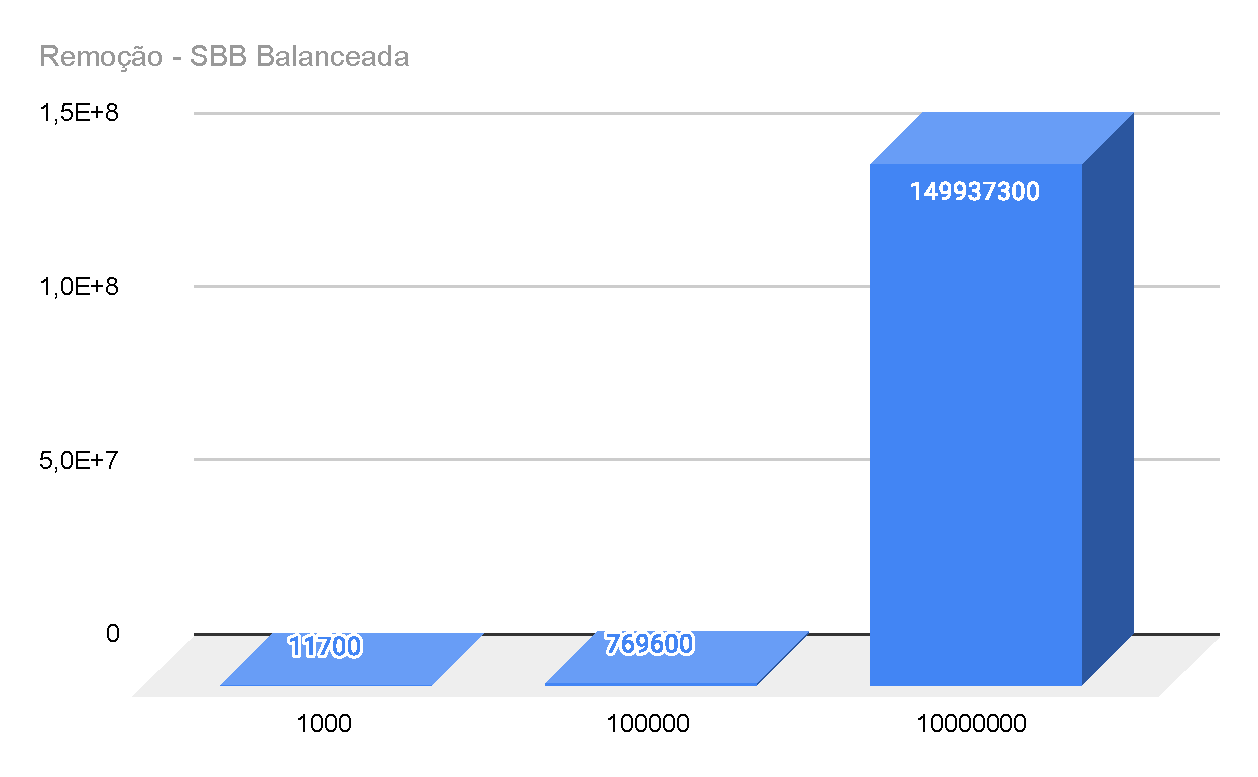
\includegraphics[scale=0.8]{Trabalho AED/fig/chart (2).pdf}
            \label{fig:Grafico 3}
    \end{center}
    
\section{Busca de elementos na TRIE}
Para a execução dos testes neste modelo de estrutura de dados foi utilizada uma implementação\cite{Samuellucas97} que recebe palavras no formato de String e as compara de acordo com seu tamanho e prioridade em ordem alfabética e facilitar a implementação de grandes quantidades de palavras foi implementado um gerador de Strings aleatórias, que utiliza de um vetor com todas as lestras do alfabeto que este método seleciona posições aleatórias do vetor e gera uma String com as letras destas posições\cite{gerarString}.

Logo os dados apresentados a seguir trazem os resultados do tempo de execução da
busca de 1\% de elementos aleatórios de TRIEs de diferentes tamanhos:

\begin{center}
        \begin{tabular}{| l | r | r | r | }
            \hline
            Quantidade de elementos & Elementos Buscados & Media de Tempo & Desvio Padrão\\
            \hline
            10\textsuperscript{3} & 100 & 1230 & 6845,509\\
            10\textsuperscript{5} & 1000 & 471,5 & 9743,600\\
            10\textsuperscript{7} & 100000 & 353,57 & 132471,980\\
            \hline
        \end{tabular}
    \end{center}

\begin{center}
            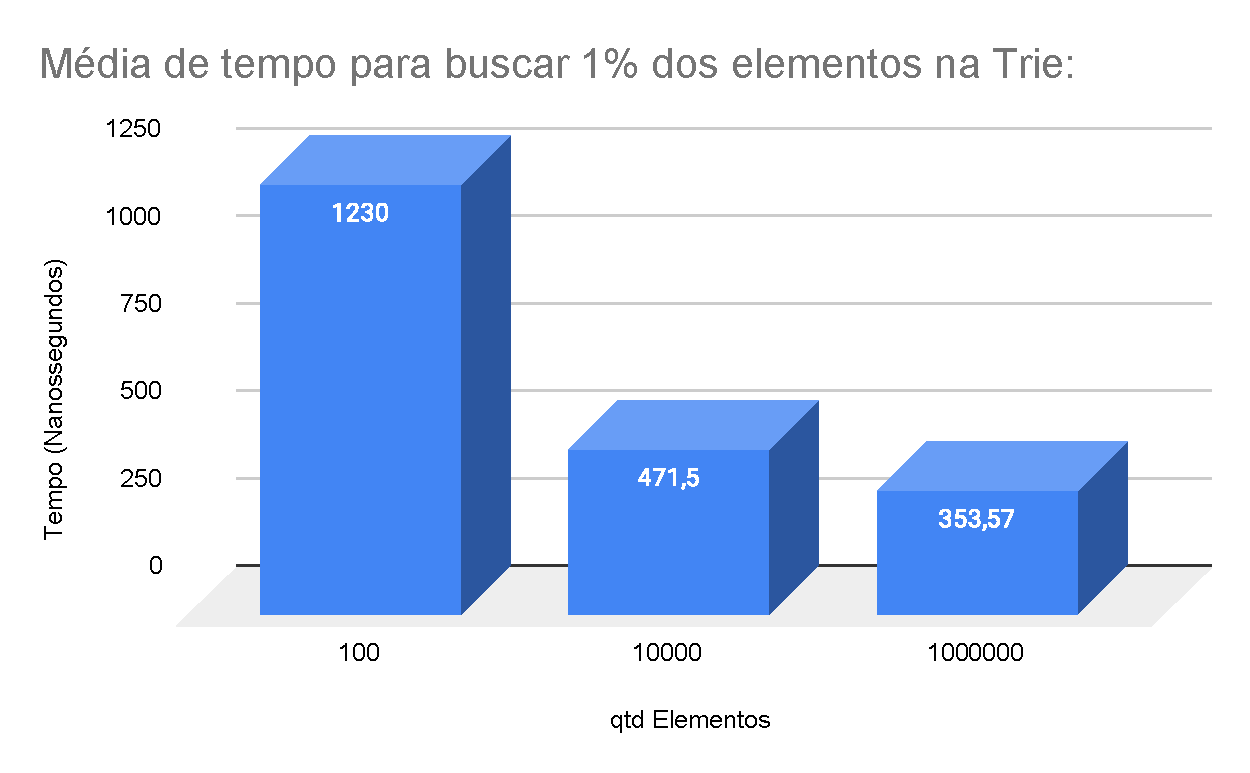
\includegraphics[scale=0.7]{Trabalho AED/fig/MediaTrie.pdf}
            \label{fig:Media de tempo Trie}
    \end{center}
    
\begin{center}
            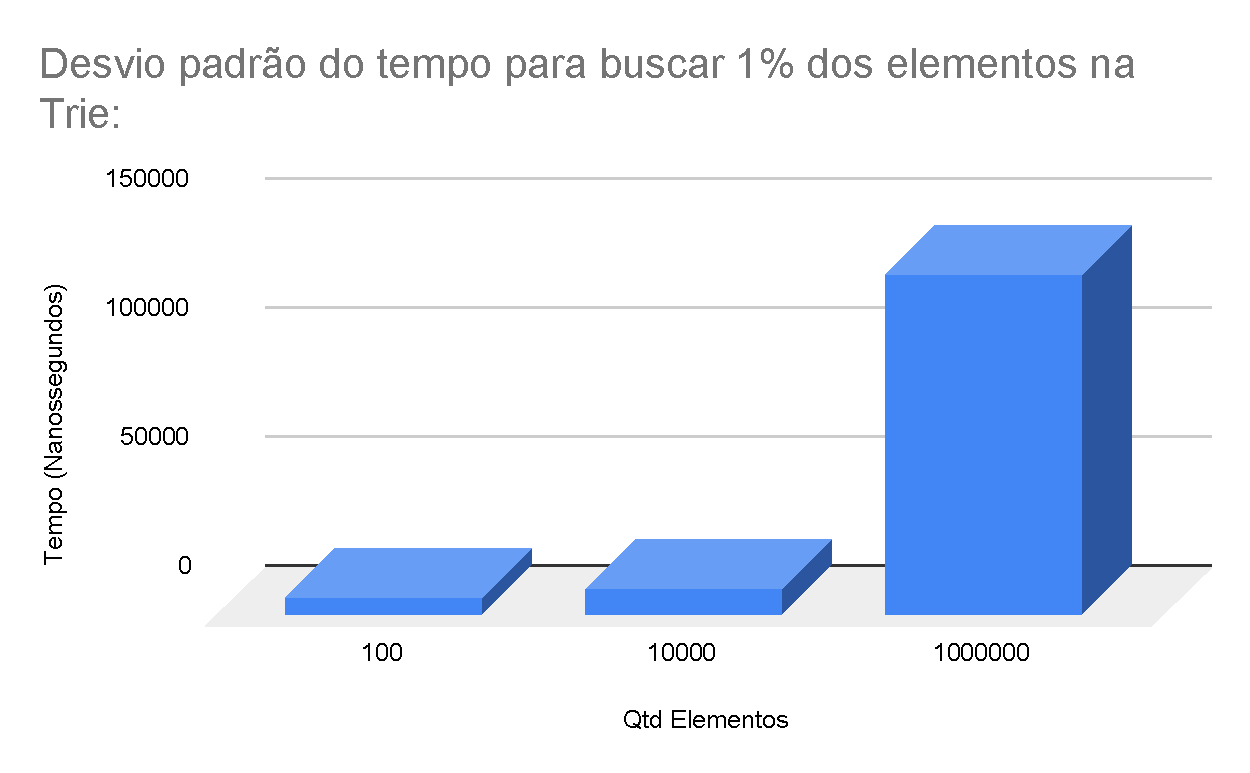
\includegraphics[scale=0.7]{Trabalho AED/fig/DesvioTrie.pdf}
            \label{fig:Media de tempo Trie}
    \end{center}

\section{busca de elementos na PATRICIA}

Para execução dos testes neste modelo de dados foi utilizado uma implementação que recebe inteiros no no formato de Interger e os compara byte a byte\cite{nivioziviani}.

Logo os dados apresentados a seguir trazem os resultados do tempo de execução da
busca de 1\% de elementos aleatórios de Patricia de diferentes tamanhos:

\begin{center}
        \begin{tabular}{| l | r | r | r | }
            \hline
            Quantidade de elementos & Elementos Buscados & Media de Tempo & Desvio Padrão\\
            \hline
            10\textsuperscript{3} & 100 & 980,0 & 2572,158626523644\\
            10\textsuperscript{5} & 1000 & 743,3 & 29827,08685071316\\
            10\textsuperscript{7} & 100000 & 448,251 & 141526,86706021812\\
            \hline
        \end{tabular}
    \end{center}
    
    \begin{center}
            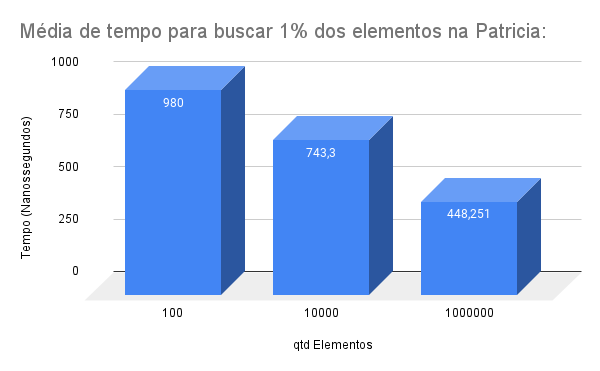
\includegraphics[scale=0.6]{Trabalho AED/fig/Média de tempo para buscar 1 dos elementos na Patricia_.png}
            \label{fig:Media de tempo Trie}
    \end{center}
    
\begin{center}
            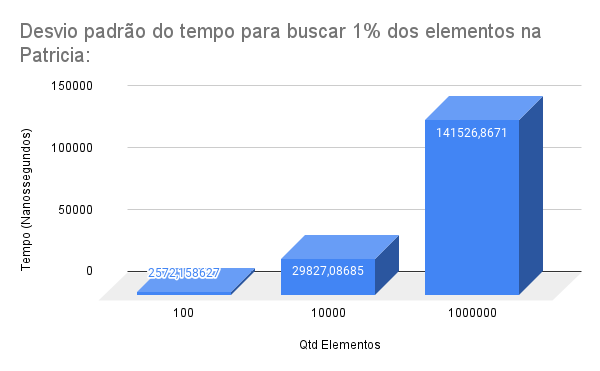
\includegraphics[scale=0.6]{Trabalho AED/fig/Desvio padrão do tempo para buscar 1 dos elementos na Patricia_.png}
            \label{fig:Media de tempo Trie}
    \end{center}



% ---
% Finaliza a parte no bookmark do PDF, para que se inicie o bookmark na raiz
% ---
\bookmarksetup{startatroot}% 
% ---

% ---
% Conclusão
% ---
\chapter[Conclusão]{Conclusão}
\label{conclusao}
%\chapter{Conclusão} - manter comentado

	\begin{flushright}
		\textit{``Palavras não bastam, não dá pra entender\\
                    E esse medo que cresce não para\\
                    É uma história que se complicou\\
                    Eu sei bem o porquê ''\\Tiê}
	    \end{flushright}
	    
	    Por fim, por meio deste trabalho foi possível além de relembrar e aprender conceitos da Física, foi possível conhecer e aplicar as ferramentas do sistema de texto LaTex.
	    Com isso é possível sim enxergar utilidade pratica neste sistema principalmente para o fator formatação, onde o texto por possuir um padrão de escrita pré definido no sistema, se formata automaticamente de acordo com o desenvolvimento do mesmo.
	    De tal forma o preconceito para com este sistema de texto deixa de existir após este trabalho.



% ----------------------------------------------------------
% ELEMENTOS PÓS-TEXTUAIS
% ----------------------------------------------------------
\postextual


% ----------------------------------------------------------
% Referências bibliográficas
% ----------------------------------------------------------
\bibliography{bibfile}



\end{document}
